
% VLDB template version of 2020-08-03 enhances the ACM template, version 1.7.0:
% https://www.acm.org/publications/proceedings-template
% The ACM Latex guide provides further information about the ACM template

\documentclass[sigconf, nonacm]{acmart}

%% The following content must be adapted for the final version
% paper-specific
\newcommand\vldbdoi{XX.XX/XXX.XX}
\newcommand\vldbpages{XXX-XXX}
% issue-specific
\newcommand\vldbvolume{14}
\newcommand\vldbissue{1}
\newcommand\vldbyear{2020}
% should be fine as it is
\newcommand\vldbauthors{\authors}
\newcommand\vldbtitle{\shorttitle} 
% leave empty if no availability url should be set
\newcommand\vldbavailabilityurl{https://doi.org/10.5281/zenodo.10701112}
% whether page numbers should be shown or not, use 'plain' for review versions, 'empty' for camera ready
\newcommand\vldbpagestyle{plain} 

\begin{document}
\title{"Duckies" Replication Package Project}

%%
%% The "author" command and its associated commands are used to define the authors and their affiliations.
\author{Oleksandr Karpenko}
\affiliation{%
  \institution{University of Passau}
  \streetaddress{Innstraße 41}
  \city{Passau}
  \state{Germany}
  \postcode{94032}
}
\email{karpen04@ads.uni-passau.de}

\maketitle

%%% do not modify the following VLDB block %%
%%% VLDB block start %%%
\ifdefempty{\vldbavailabilityurl}{}{
\vspace{.3cm}
\begingroup\small\noindent\raggedright\textbf{Artifact Availability:}\\
The source code, data, and/or other artifacts have been made available at \url{\vldbavailabilityurl}.
\endgroup
}
%%% VLDB block end %%%

\section{Introduction}

This report is about a replication package for a \textit{"Duckies"} project. \textit{"Duckies"} project based on a Chapter 3 of \textit{"Head First Data Analysis"} book \cite{Hfda}. In a chapter 3 author describes an optimization problem between two metrics. We have a company named \textit{"Bathing Friends Unlimited"}, which produces rubber ducks and fish. We have some material and time constraints in the production of both, so we need to calculate the best product mix (amount of ducks and fish to produce) for maximize profit of company. The function, which describes a problem, looks like: 
\[ c_1x_1 + c_2x_2 = P \]

Where \textit{c} is a constraint (profit for each type of product per unit), \textit{x} is a decision variable (product amount, need to find best mix), \textit{P} is an objective what we want to maximize (total profit). Later, the author also takes into account the number of ducks and fish sold recently, which adds one more constraint.

The final results are: \textbf{\textit{"Bathing Friends Unlimited"} needs to produce 150 ducks and 50 fish to receive total profit of 950\$}. I believe that if I get the same result with the same input data, the replication will be considered successful.

\section{Criteria for successful confirmation results}

I think the main criterion for successful confirmation result is a \textbf{mathematical correctness}. To fulfill this criterion, author uses a plug-in called Solver, however, I assume it is not reliable tool for replication package, because it uses commercial platform, which is unsafe in case of long-term support. Instead, I will use a library called \textit{PuLP}, a LP modeler written in Python. I assume that this library uses a mathematically correct solver, because it is popular, open-source, and has been maintained for many years.

\section{Replication package setup}
Replication package is a fully automated Docker image, based on Ubuntu Linux. For better support, I use a LTS Linux version. Docker image has all necessary tools for performing experiment, such Python with \textit{PuLP} library installed. Also, image includes LaTeX source code, which can be automatically built by Make, to get a report inside container. Detailed instructions can be found at repository page.

\section{Replication results}
\begin{figure}
  \centering
  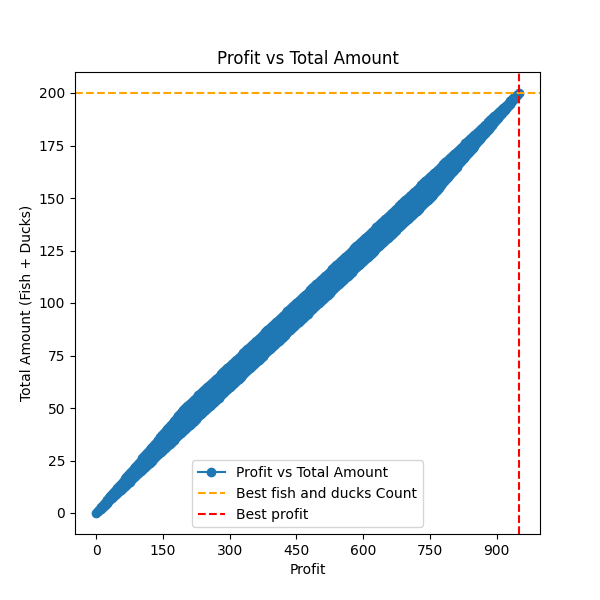
\includegraphics[width=0.5\textwidth]{figures/result_plot.png} 
  \caption{Replication result}
  \label{fig:yourlabel}
\end{figure}
 To start a replication process I execute \textit{solver\_optimization} script. It gathers all necessary values from spreadsheets and performs a linear optimization, considering what value to maximize and constraints. After execution, we receive result:
\begin{verbatim}
Optimal - objective value 950

//Some utility information

The optimal answer
---------------------------------------------------
Variable_Duck = 150.0
Variable_Fish = 50.0
\end{verbatim}
As in original experiment, \textbf{we will get an optimal profit of 950\$, if we produce 150 ducks and 50 fish}. For graphical representation, you can see the results on a Figure 1. Blue area represents all possible mixes of ducks and fish for the corresponding profit.

\section{Conclusion}
Considering the results I got from the replication process, I consider it a success. The result from book chapter and from replication package are identical. 
Despite this, some limitations and vulnerabilities remain. For example, bugs may occur in the script or in the tools we used, which may affect the purity of the experiment. If we talk about possible improvements to the replication package, I would mention scalability of the code, making it more flexible, and also exception handling.

%\clearpage

\bibliographystyle{ACM-Reference-Format}
\bibliography{sample}

\end{document}
\endinput
